\documentclass{article}
\usepackage[paperwidth=841mm,paperheight=1189mm,margin=29mm]{geometry}
\usepackage{fontspec,graphicx,xcolor,booktabs}
\usepackage[hidelinks]{hyperref}
\setmainfont{texgyreheros}[Extension=.otf,UprightFont=*-regular,BoldFont=*-bold,ItalicFont=*-italic]
\definecolor{Ink}{HTML}{152C38}
\definecolor{Accent}{HTML}{005F62}
\definecolor{Muted}{HTML}{485E67}
\definecolor{Panel}{HTML}{EAF4F2}
\definecolor{Line}{HTML}{C6D5D5}
\hypersetup{pdftitle={Credit Card Fraud Detection under a Limited Review Budget},pdfauthor={AIAA 3111 Group 20}}
\pagestyle{empty}
\setlength{\parindent}{0pt}
\raggedright
\setlength{\parskip}{5mm}
\newcommand{\body}{\fontsize{40}{53}\selectfont}
\newcommand{\smallcopy}{\fontsize{28}{37}\selectfont}
\newcommand{\heading}[1]{\par\vspace{12mm}{\color{Accent}\fontsize{48}{57}\selectfont\bfseries #1\par}\vspace{1mm}}
\newcommand{\ruleline}{\par\nointerlineskip\textcolor{Line}{\rule{\linewidth}{0.8mm}}\par}
\newcommand{\sourceurl}{https://github.com/congrenhang-ship-it/AIAA3111-Group20}
\begin{document}
\color{Ink}
\body
{\color{Accent}\fontsize{27}{34}\selectfont\bfseries AIAA 3111 \quad / \quad GROUP 20\par}
\vspace{5mm}
{\fontsize{84}{89}\selectfont\bfseries Credit Card Fraud Detection\\
under a Limited Review Budget\par}
\vspace{5mm}
{\fontsize{35}{45}\selectfont Reviewers can inspect only a fraction of transactions. Which ranking finds the most fraud at the same workload?\par}

\vspace{7mm}
\setlength{\fboxsep}{10mm}
\colorbox{Panel}{\begin{minipage}{\dimexpr\linewidth-2\fboxsep\relax}
{\color{Accent}\fontsize{61}{69}\selectfont\bfseries 64 of 74 frauds found\par}
{\fontsize{30}{39}\selectfont Weighted logistic regression reviewed 568 of 56,746 ULB test transactions. Isolation Forest found 41 frauds at the same 1\% budget.\par}
\end{minipage}}

\vspace{9mm}
\ruleline

\begin{minipage}[t]{.483\linewidth}
\body
\setlength{\parskip}{5mm}
\heading{How we compared methods}
We removed exact ULB duplicates and split transactions chronologically into training, validation and test sets. We fitted preprocessing on training data and froze model choices before testing. Each ranking sent its highest scoring 1\% of transactions for review.

We compared classifiers with distance to a K-means centroid and Isolation Forest (IF). We also mined short bin-based Apriori rules for diagnosis. Handbook and PaySim simulators let us test different inputs and transaction settings separately.

\heading{The budget changes the decision}
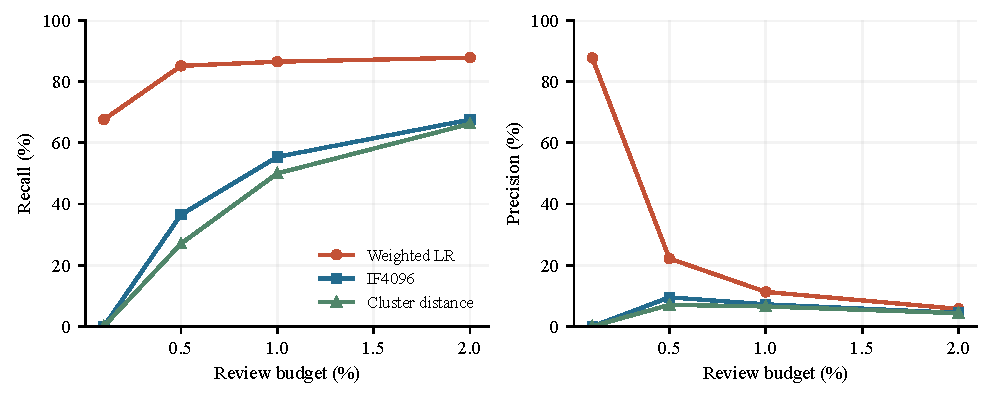
\includegraphics[width=\linewidth]{../results/figures/report_budget.pdf}\par
{\smallcopy\color{Muted}Figure 1. Recall is the share of all frauds found. Precision is the share of reviews that are fraud. All curves use the same ULB test set.\par}

At the 0.5\% budget, weighted logistic regression (LR) already found 63 frauds. Doubling the budget added one detection. At 1\%, K-means distance found 37 frauds.

\textbf{Did anomaly scores add detections?} Of the 41 frauds found by IF at 1\%, one was outside LR's list. The union needed 1,036 reviews to find 65 frauds. The combination selected before testing used LR alone.

\heading{Less supervision, more variation}
At 5\% visible training labels, LR found 55--58 frauds at the same test budget across three draws. At 25\%, it found 60--63. The full-label fit found 64.
\end{minipage}\hfill
\begin{minipage}[t]{.483\linewidth}
\body
\setlength{\parskip}{5mm}
\heading{Does extra context help?}
On Handbook's simulated test set, every model reviewed 1,458 transactions and had 1,280 frauds to find. We added past customer and terminal activity, then features from their interactions.

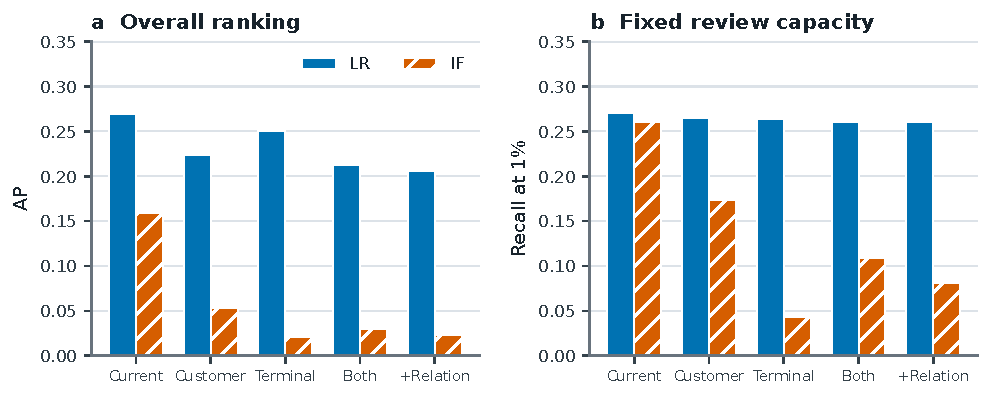
\includegraphics[width=\linewidth]{../results/figures/report_context.pdf}\par
{\smallcopy\color{Muted}Figure 2. Average precision (AP) summarizes the whole ranking. Recall at 1\% measures performance at the chosen workload.\par}

Adding both histories changed detections from 346 to 334 for LR and from 334 to 139 for IF. With 30\% of history events omitted, the history IF found 77--82 frauds across three draws.

\heading{What the rules reveal}
The first Apriori rule on ULB covered 3,846 transactions and 52 frauds. Its lift was 10.37, and 1.35\% of covered transactions were fraud. The rule points to a concentration of fraud and still covers far more transactions than the review team can handle.

\heading{A different ranking on PaySim}
At 1,289 reviews, IF detected 102 of 413 frauds. Amount ranking detected 94 and had the highest AP (0.0798). Weighted LR detected 80.

\end{minipage}

\vspace{12mm}
\ruleline
\heading{What to take into practice}
Set review capacity first. Compare how many frauds the list catches, then use AP to examine the full ranking. Test whether historical features improve the list before adding them.

{\smallcopy\color{Muted}Evidence comes from one chronological ULB split with 74 test frauds and two simulated datasets.\par}

\vfill
\ruleline
{\smallcopy\color{Muted}
Data: ULB/Worldline (Zenodo), Fraud Detection Handbook simulator and PaySim (López-Rojas et al.). Figures and counts are from the formal test results.\par
\href{\sourceurl}{\textbf{Report, code and data sources on GitHub}} \quad / \quad github.com/congrenhang-ship-it/AIAA3111-Group20\par}
\end{document}
